\documentclass[aspectratio=169,8pt]{beamer}

\usepackage[T1]{fontenc}
\usepackage{helvet}
\renewcommand{\familydefault}{\sfdefault}
\usepackage{graphicx}
\usepackage{tikz}
\usetikzlibrary{arrows.meta,positioning,calc,shapes.geometric}
\usepackage{booktabs}
\usepackage{tabularx}
\usepackage{array}
\usepackage{amsmath}
\usepackage{xcolor}
\usepackage{hyperref}
\usepackage{ragged2e}

\definecolor{Navy}{HTML}{0B1F33}
\definecolor{Teal}{HTML}{16A6A3}
\definecolor{Gold}{HTML}{D99A1E}
\definecolor{Light}{HTML}{F8FAFA}
\definecolor{Line}{HTML}{D8E1E5}
\definecolor{SoftTeal}{HTML}{E6F7F6}
\definecolor{SoftGold}{HTML}{FFF4DF}
\definecolor{RedSoft}{HTML}{FBE9E7}
\definecolor{Danger}{HTML}{C94C4C}
\definecolor{Muted}{HTML}{61717D}

\newcolumntype{Y}{>{\RaggedRight\arraybackslash}X}

\setbeamercolor{background canvas}{bg=Light}
\setbeamercolor{normal text}{fg=Navy}
\setbeamercolor{frametitle}{fg=Navy}
\setbeamerfont{frametitle}{series=\bfseries,size=\Large}
\setbeamertemplate{navigation symbols}{}
\setbeamersize{text margin left=0.55cm,text margin right=0.55cm}
\hypersetup{colorlinks=true,linkcolor=Teal,urlcolor=Teal}

\newcommand{\slidetitle}[1]{\vspace{-0.2cm}\frametitle{#1}}
\newcommand{\repo}{\href{https://github.com/sorooshaghaei/Project_final_master1}{github.com/sorooshaghaei/Project\_final\_master1}}
\newcommand{\pill}[2]{%
\tikz[baseline=(X.base)]\node[rounded corners=2pt,fill=#1,inner xsep=4pt,inner ysep=2pt] (X) {\scriptsize\bfseries #2};}

\newcommand{\metriccard}[3]{%
\begin{minipage}[t]{#1}
\centering
\setlength{\fboxsep}{4pt}%
\setlength{\fboxrule}{0.45pt}%
\fcolorbox{Line}{white}{\begin{minipage}{\dimexpr#1-11pt\relax}
\centering\scriptsize #2\\[2pt]{\Large\bfseries\color{Teal}#3}
\end{minipage}}
\end{minipage}}

\newcommand{\slideimage}[2][0.95\linewidth]{%
\includegraphics[width=#1,height=0.52\textheight,keepaspectratio]{#2}}

\newcommand{\warnbox}[1]{%
\begin{tikzpicture}
\node[draw=Gold,rounded corners=4pt,fill=SoftGold,inner sep=5pt,text width=0.90\linewidth,align=left] {\small #1};
\end{tikzpicture}}

\newcommand{\TotalFrames}{24}
\newcommand{\NavButtons}{%
\ifnum\value{framenumber}>1%
\hyperlink{slide\number\numexpr\value{framenumber}-1\relax}{\beamerbutton{Prev}}%
\else{\color{Muted}\beamerbutton{Prev}}%
\fi%
\hspace{0.07cm}%
\ifnum\value{framenumber}<\TotalFrames%
\hyperlink{slide\number\numexpr\value{framenumber}+1\relax}{\beamerbutton{Next}}%
\else{\color{Muted}\beamerbutton{Next}}%
\fi}

\setbeamertemplate{footline}{%
\leavevmode%
\hbox{%
\begin{beamercolorbox}[wd=\paperwidth,ht=3.2ex,dp=1.3ex,leftskip=0.55cm,rightskip=0.55cm]{normal text}%
{\scriptsize\color{Muted}\insertframenumber{} / \TotalFrames}\hfill{\scriptsize\NavButtons}
\end{beamercolorbox}}}

\tikzset{
 block/.style={draw=Line, rounded corners=4pt, fill=white, minimum height=0.95cm, align=center, inner sep=4pt, font=\scriptsize},
 tealblock/.style={block, draw=Teal, fill=SoftTeal},
 goldblock/.style={block, draw=Gold, fill=SoftGold},
 arrow/.style={-Latex, thick, draw=Navy},
 thinarrow/.style={-Latex, draw=Muted}
}

\begin{document}

% 1
\begin{frame}[label=slide1]
\vspace{0.25cm}
\begin{columns}[T,totalwidth=\linewidth]
\begin{column}{0.50\linewidth}
{\Huge\bfseries Self-Supervised Test-Time Training}\\[0.12cm]
{\Large\color{Muted}Activation Matching for CIFAR-10-C Distribution Shift}\\[0.45cm]
\pill{SoftTeal}{TER M1 VMI Final Project 2026}\quad\pill{SoftGold}{Université Paris Cité}\\[0.55cm]
{\large Rayane KHATIM \;--\; Mehdi AGHAEI}\\[0.3cm]
{\small Repository: \repo}
\end{column}
\begin{column}{0.45\linewidth}
\centering

\includegraphics[width=0.62\linewidth]{assets/universite_paris_cite_logo.png}\\[0.28cm]
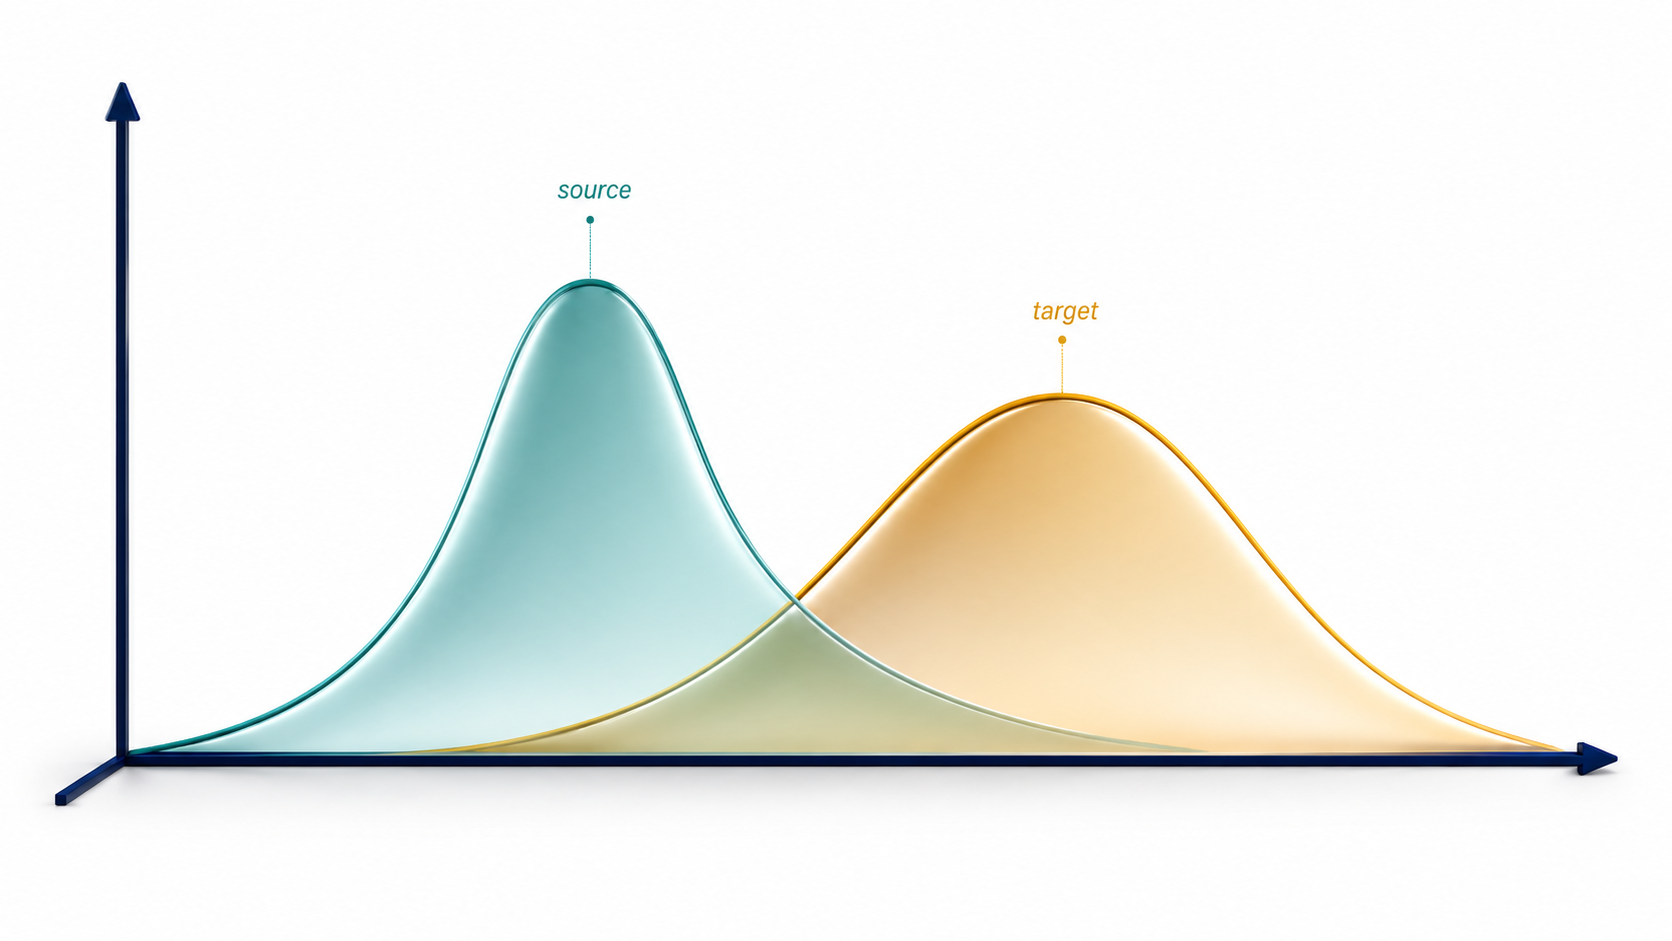
\includegraphics[width=\linewidth,height=0.50\textheight,keepaspectratio]{assets/1.png}
\end{column}
\end{columns}
\end{frame}

% 2
\begin{frame}[label=slide2]
\slidetitle{Executive Summary}
\begin{columns}[T,totalwidth=\linewidth]
\begin{column}{0.31\linewidth}
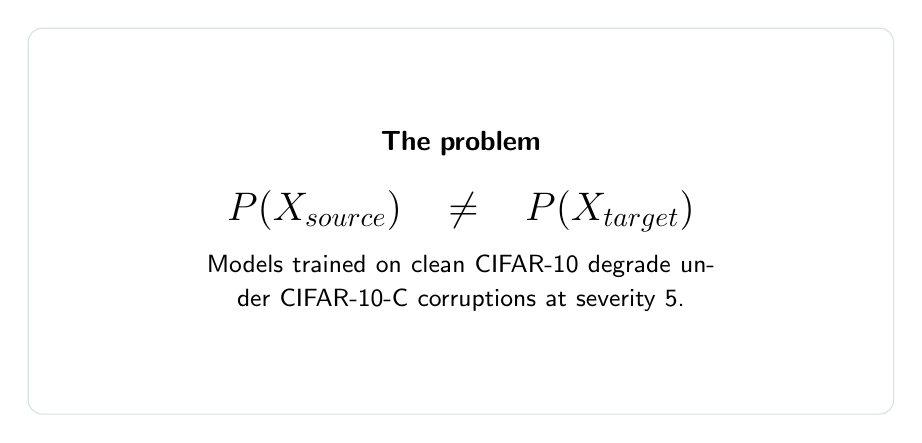
\begin{tikzpicture}
\node[draw=Line,rounded corners=5pt,fill=white,text width=0.86\linewidth,minimum height=4.9cm,inner sep=8pt,align=center] {
{\bfseries The problem}\\[0.25cm]
\Large $P(X_{source}) \neq P(X_{target})$\\[0.25cm]
\small Models trained on clean CIFAR-10 degrade under CIFAR-10-C corruptions at severity 5.
};
\end{tikzpicture}
\end{column}
\begin{column}{0.31\linewidth}
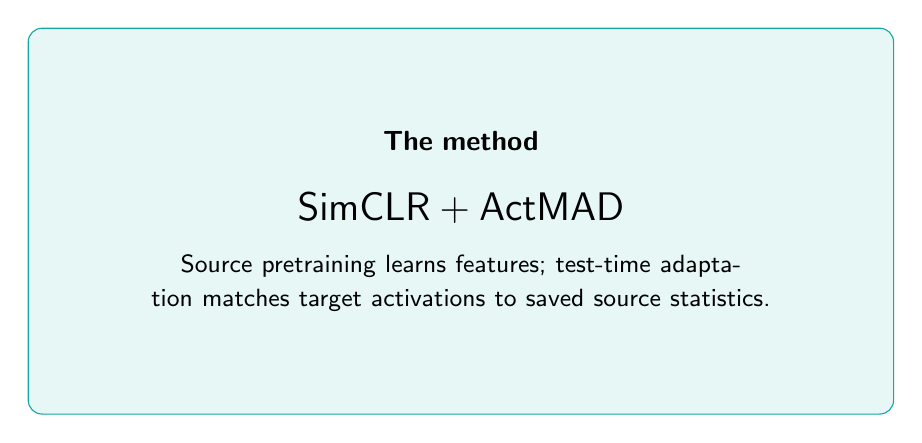
\begin{tikzpicture}
\node[draw=Teal,rounded corners=5pt,fill=SoftTeal,text width=0.86\linewidth,minimum height=4.9cm,inner sep=8pt,align=center] {
{\bfseries The method}\\[0.25cm]
\Large SimCLR $+$ ActMAD\\[0.25cm]
\small Source pretraining learns features; test-time adaptation matches target activations to saved source statistics.
};
\end{tikzpicture}
\end{column}
\begin{column}{0.31\linewidth}
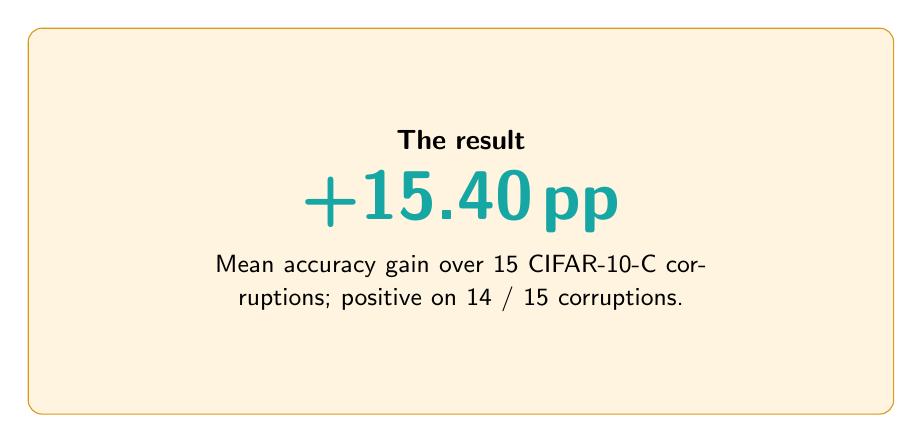
\begin{tikzpicture}
\node[draw=Gold,rounded corners=5pt,fill=SoftGold,text width=0.86\linewidth,minimum height=4.9cm,inner sep=8pt,align=center] {
{\bfseries The result}\\[0.25cm]
{\Huge\bfseries\color{Teal}+15.40 pp}\\[0.25cm]
\small Mean accuracy gain over 15 CIFAR-10-C corruptions; positive on 14 / 15 corruptions.
};
\end{tikzpicture}
\end{column}
\end{columns}
\end{frame}

% 3
\begin{frame}[label=slide3]
\slidetitle{Motivation and Context}
\begin{columns}[T,totalwidth=\linewidth]
\begin{column}{0.35\linewidth}
{\small
\begin{itemize}\setlength\itemsep{0.25cm}
\item The repository targets \textbf{test-time training} under distribution shift.
\item Source training uses clean CIFAR-10; target evaluation uses CIFAR-10-C corruptions.
\item Adaptation must work without target labels during deployment.
\item The project compares static inference against ActMAD adaptation on corrupted target batches.
\end{itemize}
}
\end{column}
\begin{column}{0.65\linewidth}
\centering
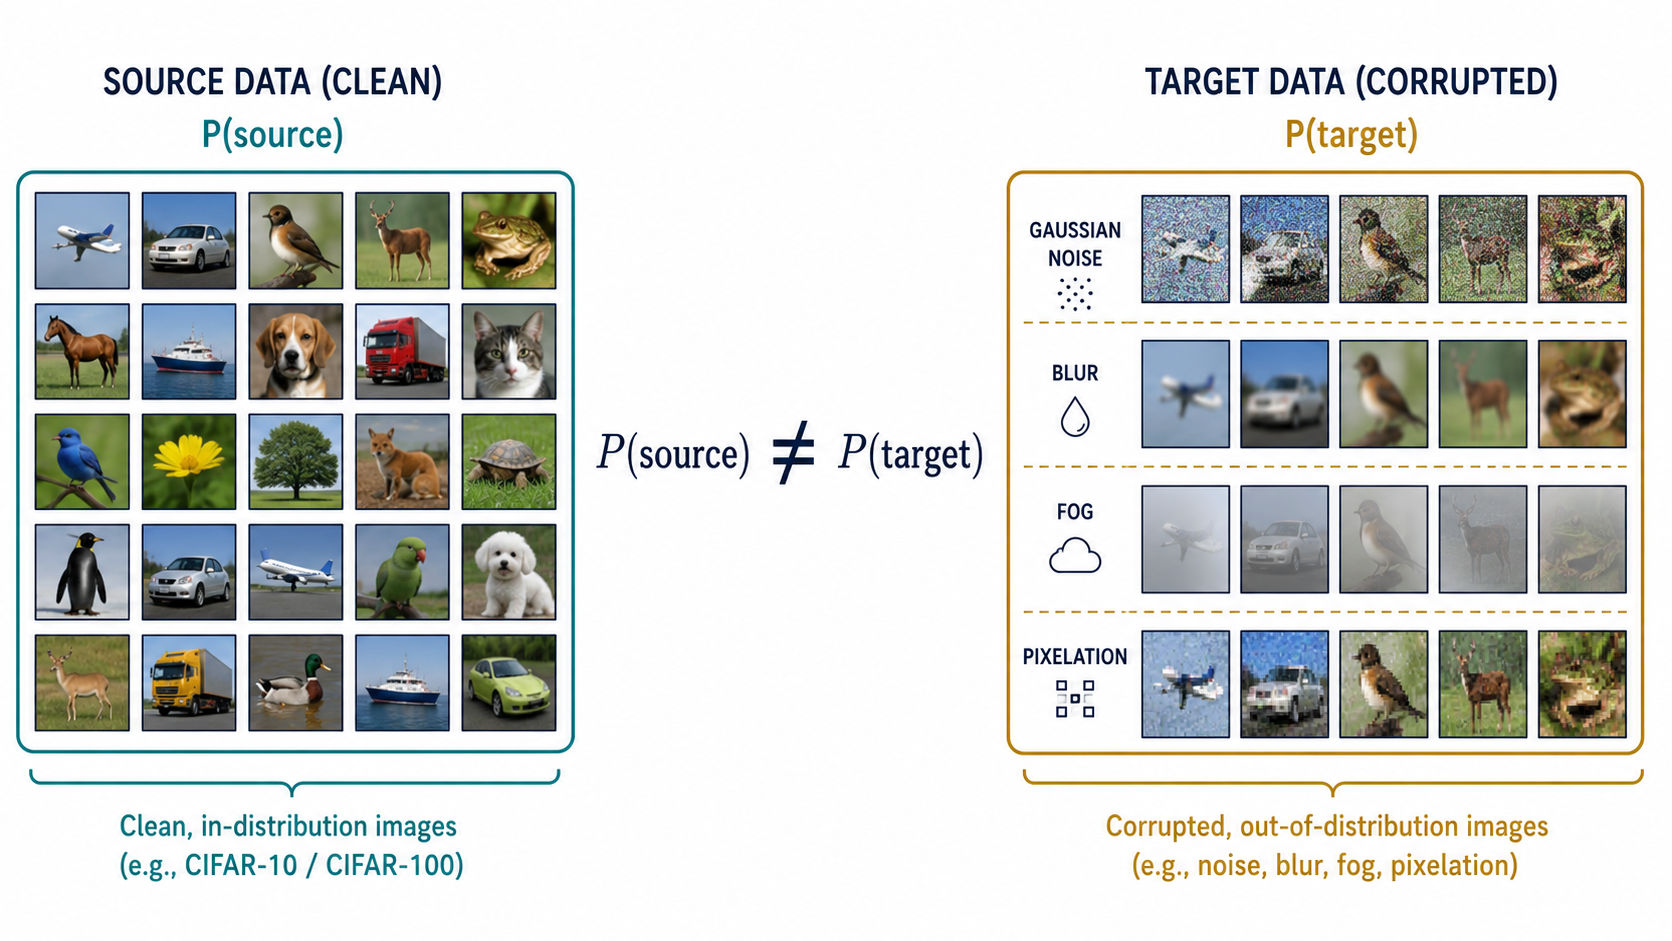
\includegraphics[width=\linewidth,height=0.75\textheight,keepaspectratio]{assets/2.png}
\end{column}
\end{columns}
\end{frame}

% 4
\begin{frame}[label=slide4]
\slidetitle{Problem Definition}
\begin{center}
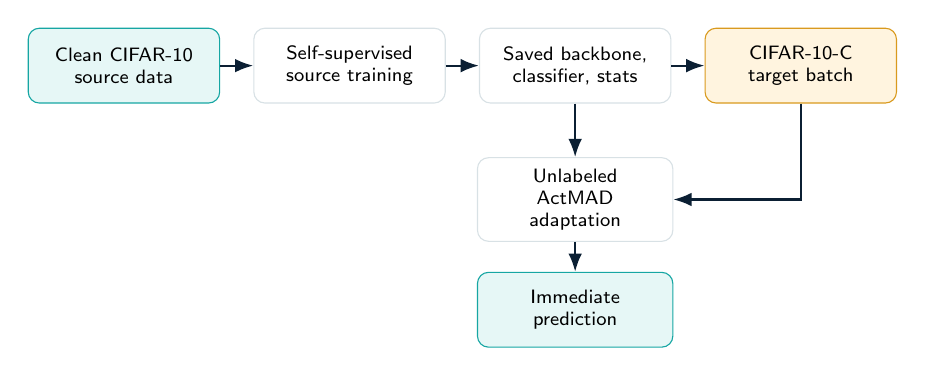
\begin{tikzpicture}[node distance=0.38cm and 0.42cm]
\node[tealblock,text width=2.15cm] (source) {Clean CIFAR-10\\source data};
\node[block,text width=2.15cm,right=of source] (train) {Self-supervised\\source training};
\node[block,text width=2.15cm,right=of train] (stats) {Saved backbone,\\classifier, stats};
\node[goldblock,text width=2.15cm,right=of stats] (target) {CIFAR-10-C\\target batch};
\node[block,text width=2.2cm,below=0.68cm of stats] (adapt) {Unlabeled\\ActMAD adaptation};
\node[tealblock,text width=2.2cm,below=0.38cm of adapt] (pred) {Immediate\\prediction};
\draw[arrow] (source) -- (train);
\draw[arrow] (train) -- (stats);
\draw[arrow] (stats) -- (target);
\draw[arrow] (target.south) |- (adapt.east);
\draw[arrow] (stats) -- (adapt);
\draw[arrow] (adapt) -- (pred);
\end{tikzpicture}
\end{center}
\vspace{0.05cm}
\begin{columns}[T,totalwidth=0.94\linewidth]
\begin{column}{0.47\linewidth}
\textbf{Input}\quad unlabeled corrupted target batch\\[0.18cm]
\textbf{Constraint}\quad no target labels during adaptation
\end{column}
\begin{column}{0.47\linewidth}
\textbf{Output}\quad class logits and accuracy\\[0.18cm]
\textbf{Mechanism}\quad ActMAD activation matching
\end{column}
\end{columns}
\vspace{0.18cm}
\small The code evaluates whether batch-wise adaptation improves top-1 accuracy relative to the frozen baseline.
\end{frame}

% 5
\begin{frame}[label=slide5]
\slidetitle{Research and Engineering Objectives}
\begin{columns}[T,totalwidth=\linewidth]
\begin{column}{0.48\linewidth}
\begin{enumerate}\setlength\itemsep{0.22cm}
\item Build a SimCLR-based feature extractor on CIFAR-10.
\item Save reusable artifacts: backbone, classifier, source activation statistics.
\item Implement batch-wise ActMAD test-time adaptation.
\item Evaluate baseline vs adapted inference on CIFAR-10-C severity 5.
\end{enumerate}
\end{column}
\begin{column}{0.48\linewidth}
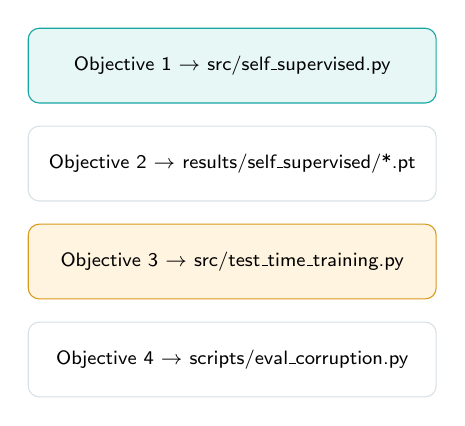
\begin{tikzpicture}[node distance=0.28cm]
\node[tealblock,text width=4.9cm] (a) {Objective 1 $\rightarrow$ src/self\_supervised.py};
\node[block,text width=4.9cm,below=of a] (b) {Objective 2 $\rightarrow$ results/self\_supervised/*.pt};
\node[goldblock,text width=4.9cm,below=of b] (c) {Objective 3 $\rightarrow$ src/test\_time\_training.py};
\node[block,text width=4.9cm,below=of c] (d) {Objective 4 $\rightarrow$ scripts/eval\_corruption.py};
\end{tikzpicture}
\end{column}
\end{columns}
\end{frame}

% 6
\begin{frame}[label=slide6]
\slidetitle{Dataset, Inputs, Experimental Material}
\centering
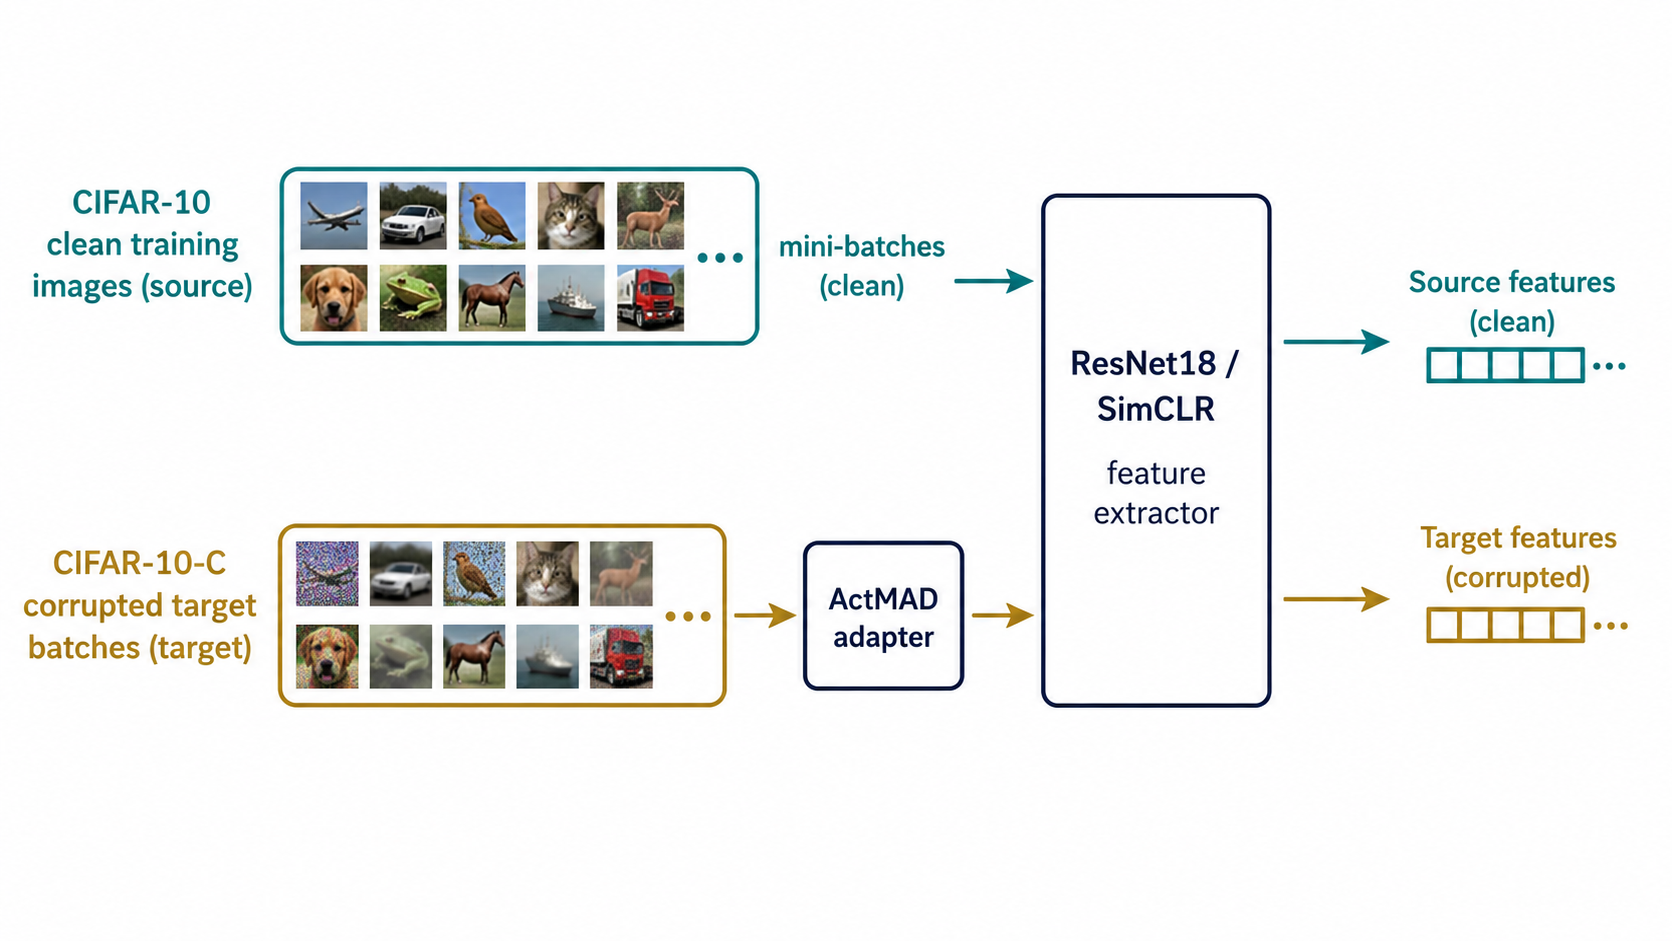
\includegraphics[width=\linewidth,height=0.65\textheight,keepaspectratio]{assets/3.png}
\vfill
{\small
\renewcommand{\arraystretch}{1.12}
\begin{tabularx}{1.0\linewidth}{>{\bfseries\RaggedRight\arraybackslash}p{2.25cm}Y}
Source data & CIFAR-10 train split via torchvision \\
Target data & CIFAR-10-C official .npy files \\
Corruptions & 15 CIFAR-10-C corruptions \\
Severity & 5 \\
Batch size & 16 for TTT evaluation \\
Samples & 10,000 per corruption slice \\
\end{tabularx}
}
\end{frame}

% 7
\begin{frame}[label=slide7]
\slidetitle{Global Method Overview}
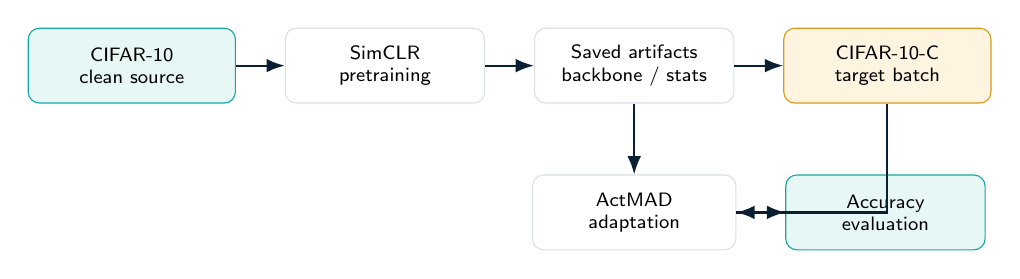
\begin{tikzpicture}[node distance=0.42cm and 0.62cm]
\node[tealblock,text width=2.35cm] (cifar) {CIFAR-10\\clean source};
\node[block,text width=2.25cm,right=of cifar] (simclr) {SimCLR\\pretraining};
\node[block,text width=2.25cm,right=of simclr] (art) {Saved artifacts\\backbone / stats};
\node[goldblock,text width=2.35cm,right=of art] (cifarC) {CIFAR-10-C\\target batch};
\node[block,text width=2.3cm,below=0.9cm of art] (actmad) {ActMAD\\adaptation};
\node[tealblock,text width=2.25cm,right=of actmad] (eval) {Accuracy\\evaluation};
\draw[arrow] (cifar) -- (simclr);
\draw[arrow] (simclr) -- (art);
\draw[arrow] (art) -- (cifarC);
\draw[arrow] (cifarC) |- (actmad);
\draw[arrow] (art) -- (actmad);
\draw[arrow] (actmad) -- (eval);
\end{tikzpicture}
\vspace{0.45cm}
\begin{columns}[T,totalwidth=\linewidth]
\begin{column}{0.31\linewidth}\metriccard{\linewidth}{Pretraining}{SimCLR}\end{column}
\begin{column}{0.31\linewidth}\metriccard{\linewidth}{Target adaptation}{ActMAD}\end{column}
\begin{column}{0.31\linewidth}\metriccard{\linewidth}{Evaluation}{15 corruptions}\end{column}
\end{columns}
\end{frame}

% 8
\begin{frame}[label=slide8]
\slidetitle{Core Technical Mechanism}
\begin{columns}[T,totalwidth=\linewidth]
\begin{column}{0.40\linewidth}
{\small
\textbf{SimCLR source stage}\\[-1mm]
\[
\mathcal{L}_{NT\text{-}Xent} = \mathrm{CE}\left(\frac{zz^\top}{\tau}, y_{pos}\right)
\]
\vspace{-0.15cm}
\textbf{ActMAD target stage}\\[-1mm]
\[
\mathcal{L}_{ActMAD}=\frac{1}{L}\sum_{\ell}\left(\lVert\mu_t^\ell-\mu_s^\ell\rVert_2^2+\lVert\sigma_t^\ell-\sigma_s^\ell\rVert_2^2\right)
\]
\small ActMAD updates only normalization-layer parameters during the target-batch adaptation loop.
}
\end{column}
\begin{column}{0.58\linewidth}
\centering
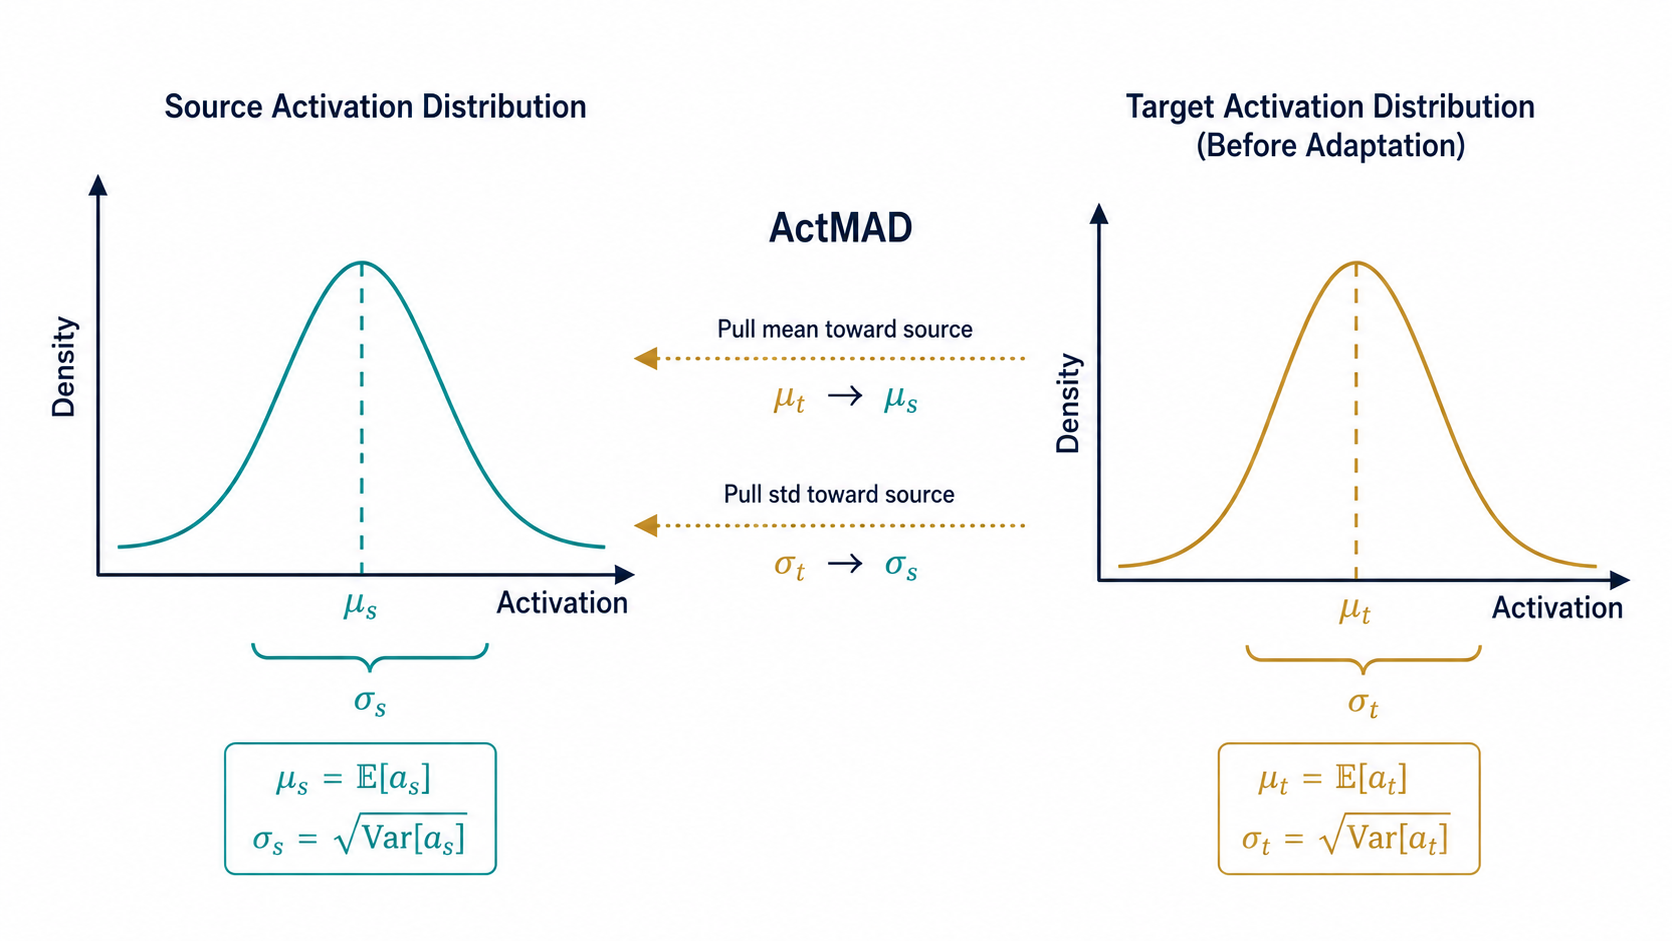
\includegraphics[width=\linewidth,height=0.58\textheight,keepaspectratio]{assets/4.png}
\end{column}
\end{columns}
\end{frame}

% 9
\begin{frame}[label=slide9]
\slidetitle{Architecture and Software Pipeline}
\begin{columns}[T,totalwidth=\linewidth]
\begin{column}{0.44\linewidth}
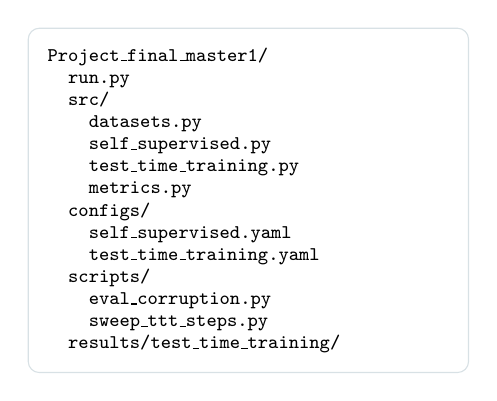
\begin{tikzpicture}[font=\scriptsize]
\node[draw=Line,rounded corners=4pt,fill=white,inner sep=7pt,text width=5.1cm,align=left] {
\texttt{Project\_final\_master1/}\\
\quad\texttt{run.py}\\
\quad\texttt{src/}\\
\quad\quad\texttt{datasets.py}\\
\quad\quad\texttt{self\_supervised.py}\\
\quad\quad\texttt{test\_time\_training.py}\\
\quad\quad\texttt{metrics.py}\\
\quad\texttt{configs/}\\
\quad\quad\texttt{self\_supervised.yaml}\\
\quad\quad\texttt{test\_time\_training.yaml}\\
\quad\texttt{scripts/}\\
\quad\quad\texttt{eval\_corruption.py}\\
\quad\quad\texttt{sweep\_ttt\_steps.py}\\
\quad\texttt{results/test\_time\_training/}
};
\end{tikzpicture}
\end{column}
\begin{column}{0.52\linewidth}
\begin{itemize}\setlength\itemsep{0.22cm}
\item \texttt{run.py}: unified entry point with task aliases \texttt{ssl} and \texttt{ttt}.
\item \texttt{src/self\_supervised.py}: SimCLR model, projection head, NT-Xent loss, linear evaluation.
\item \texttt{src/test\_time\_training.py}: activation hooks, source stats, ActMAD loss, TTT adapter.
\item \texttt{scripts/}: all-corruption evaluation and step sweep.
\end{itemize}
\end{column}
\end{columns}
\end{frame}

% 10
\begin{frame}[label=slide10]
\slidetitle{Implementation Details}
\begin{columns}[T,totalwidth=\linewidth]
\begin{column}{0.48\linewidth}
{\small
\renewcommand{\arraystretch}{1.12}
\begin{tabularx}{\linewidth}{>{\bfseries\RaggedRight\arraybackslash}p{2.1cm}Y}
Language & Python \\
Core stack & PyTorch, torchvision, NumPy, PyYAML \\
Backbone & ResNet18 adapted for 32$\times$32 CIFAR images \\
SSL output & backbone, classifier, source stats \\
TTT output & baseline / ActMAD accuracy \\
Seed & 42 in main configs \\
Hardware & Not provided in the repository \\
\end{tabularx}
}
\end{column}
\begin{column}{0.48\linewidth}
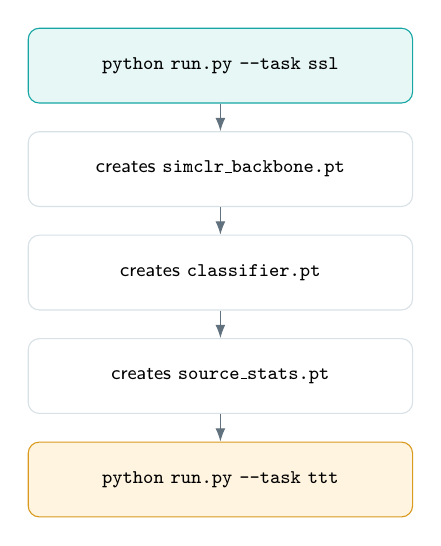
\begin{tikzpicture}[node distance=0.35cm]
\node[tealblock,text width=4.6cm] (a) {\texttt{python run.py --task ssl}};
\node[block,text width=4.6cm,below=of a] (b) {creates \texttt{simclr\_backbone.pt}};
\node[block,text width=4.6cm,below=of b] (c) {creates \texttt{classifier.pt}};
\node[block,text width=4.6cm,below=of c] (d) {creates \texttt{source\_stats.pt}};
\node[goldblock,text width=4.6cm,below=of d] (e) {\texttt{python run.py --task ttt}};
\draw[thinarrow] (a) -- (b);\draw[thinarrow] (b) -- (c);\draw[thinarrow] (c) -- (d);\draw[thinarrow] (d) -- (e);
\end{tikzpicture}
\end{column}
\end{columns}
\end{frame}

% 11
\begin{frame}[label=slide11]
\slidetitle{Experimental Setup}
\begin{center}
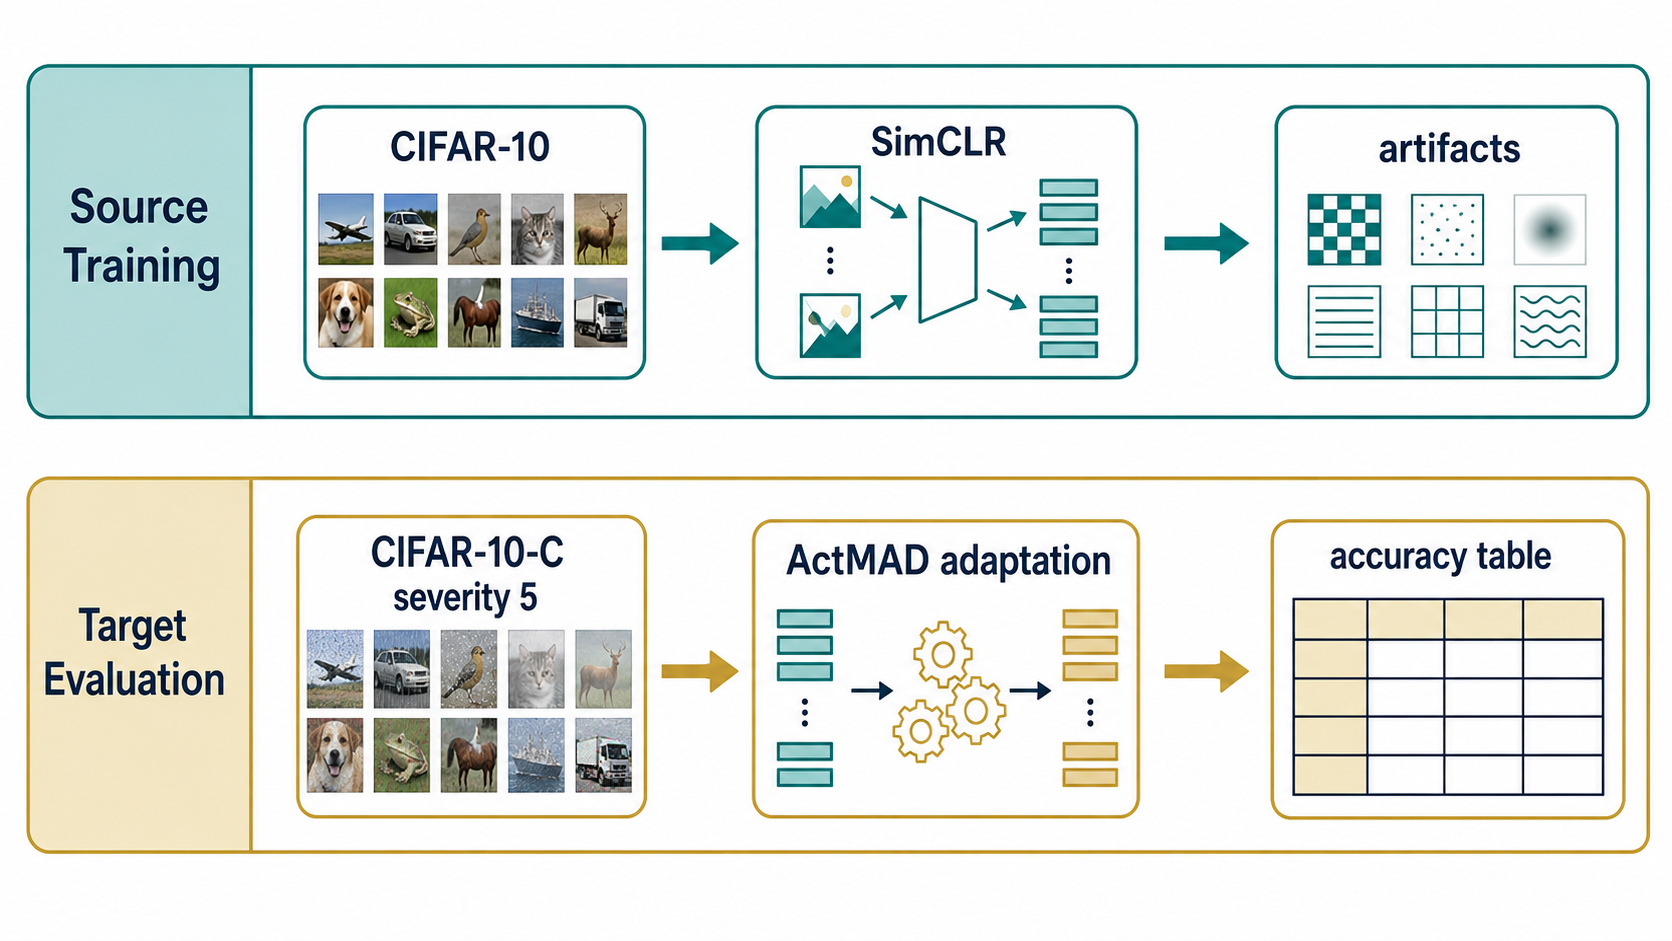
\includegraphics[width=\linewidth,height=0.55\textheight,keepaspectratio]{assets/5.png}
\end{center}
\vspace{0.08cm}
\begin{columns}[T,totalwidth=\linewidth]
\begin{column}{0.49\linewidth}
{\small
\textbf{Source / SimCLR}\\[0.05cm]
\renewcommand{\arraystretch}{1.12}
\begin{tabularx}{\linewidth}{>{\bfseries\RaggedRight\arraybackslash}p{2.25cm}Y}
Method & SimCLR \\
Epochs & 200 \\
Batch size & 256 \\
Learning rate & 0.03 \\
Backbone & ResNet18 \\
Projection dim & 128 default in code \\
\end{tabularx}
}
\end{column}
\begin{column}{0.49\linewidth}
{\small
\textbf{Target / ActMAD}\\[0.05cm]
\renewcommand{\arraystretch}{1.12}
\begin{tabularx}{\linewidth}{>{\bfseries\RaggedRight\arraybackslash}p{2.25cm}Y}
Method & ActMAD \\
Steps & 10 per batch \\
Learning rate & 0.0001 \\
Target corruption & all 15 in full eval; shot\_noise in config \\
Severity & 5 \\
Metric & Top-1 accuracy \\
\end{tabularx}
}
\end{column}
\end{columns}
\end{frame}

% 12
\begin{frame}[label=slide12]
\slidetitle{Metrics}
\begin{columns}[T,totalwidth=\linewidth]
\begin{column}{0.48\linewidth}
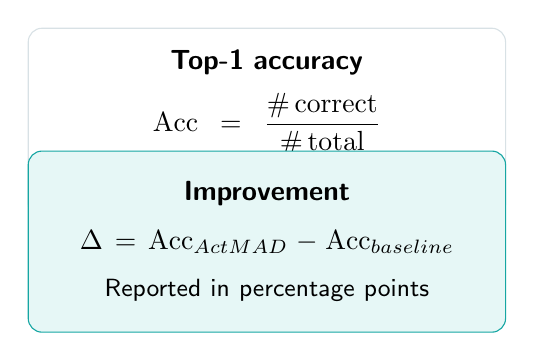
\begin{tikzpicture}
\node[draw=Line,rounded corners=5pt,fill=white,text width=5.5cm,minimum height=2.3cm,inner sep=8pt,align=center] {
\textbf{Top-1 accuracy}\\[0.2cm]
$\displaystyle \mathrm{Acc}=\frac{\#\,\mathrm{correct}}{\#\,\mathrm{total}}$\\[0.18cm]
\small Implemented in \texttt{src/metrics.py}
};
\node[draw=Teal,rounded corners=5pt,fill=SoftTeal,text width=5.5cm,minimum height=2.3cm,inner sep=8pt,align=center,below=0.35cm] {
\textbf{Improvement}\\[0.2cm]
$\displaystyle \Delta=\mathrm{Acc}_{ActMAD}-\mathrm{Acc}_{baseline}$\\[0.18cm]
\small Reported in percentage points
};
\end{tikzpicture}
\end{column}
\begin{column}{0.48\linewidth}
\begin{itemize}\setlength\itemsep{0.23cm}
\item Baseline: prediction with the frozen source-trained model.
\item ActMAD: prediction after unlabeled batch adaptation.
\item All-corruption output: per-corruption accuracy and improvement.
\item Step sweep output: accuracy at 3, 5, and 10 adaptation steps.
\end{itemize}
\end{column}
\end{columns}
\end{frame}

% 13
\begin{frame}[label=slide13]
\slidetitle{Main Quantitative Results}
\begin{columns}[T,totalwidth=\linewidth]
\begin{column}{0.45\linewidth}
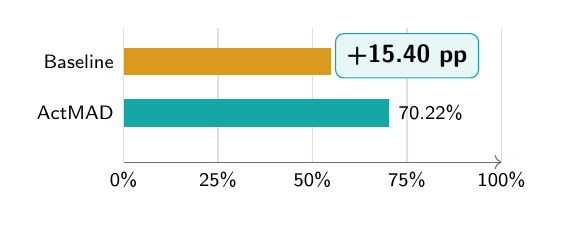
\begin{tikzpicture}[x=0.048cm,y=1cm]
\draw[->,draw=Muted] (0,0) -- (100,0);
\foreach \x in {0,25,50,75,100}{\draw[draw=Line] (\x,0) -- (\x,1.7); \node[below] at (\x,0) {\scriptsize \x\%};}
\fill[Gold] (0,1.1) rectangle (54.82,1.45);
\fill[Teal] (0,0.45) rectangle (70.22,0.80);
\node[left] at (0,1.275) {\scriptsize Baseline};
\node[left] at (0,0.625) {\scriptsize ActMAD};
\node[right] at (54.82,1.275) {\scriptsize 54.82\%};
\node[right] at (70.22,0.625) {\scriptsize 70.22\%};
\node[draw=Teal,rounded corners=3pt,fill=SoftTeal,inner sep=4pt] at (75,1.35) {\small\bfseries +15.40 pp};
\end{tikzpicture}
\vspace{0.25cm}
{\small
\begin{tabular}{@{}>{\bfseries}l l@{}}
Positive & 14 / 15 corruptions \\
Negative & brightness, -1.55 pp \\
Best gain & impulse\_noise, +41.59 pp \\
\end{tabular}
}
\end{column}
\begin{column}{0.47\linewidth}
{\scriptsize
\begin{tabular}{@{}lrr@{}}
\toprule
Corruption & Base & ActMAD \\
\midrule
impulse\_noise & 17.89 & 59.48 \\
gaussian\_noise & 27.36 & 68.02 \\
shot\_noise & 33.02 & 69.09 \\
pixelate & 38.71 & 67.32 \\
brightness & 82.21 & 80.66 \\
\bottomrule
\end{tabular}
}
\vspace{0.18cm}
{\scriptsize Accuracy in percent; full table in \texttt{corruption\_eval.csv}.}
\end{column}
\end{columns}
\end{frame}

% 14
\begin{frame}[label=slide14]
\slidetitle{Result Interpretation}
\begin{columns}[T,totalwidth=\linewidth]
\begin{column}{0.40\linewidth}
\begin{itemize}\setlength\itemsep{0.25cm}
\item ActMAD is strongest on noise-like shifts: impulse, Gaussian, and shot noise.
\item Gains remain positive but smaller on blur and compression shifts.
\item Brightness is the single degradation case, suggesting that matching activation moments is not universally safe.
\item The average gain is large, but the method remains corruption-dependent.
\end{itemize}
\end{column}
\begin{column}{0.58\linewidth}
\centering
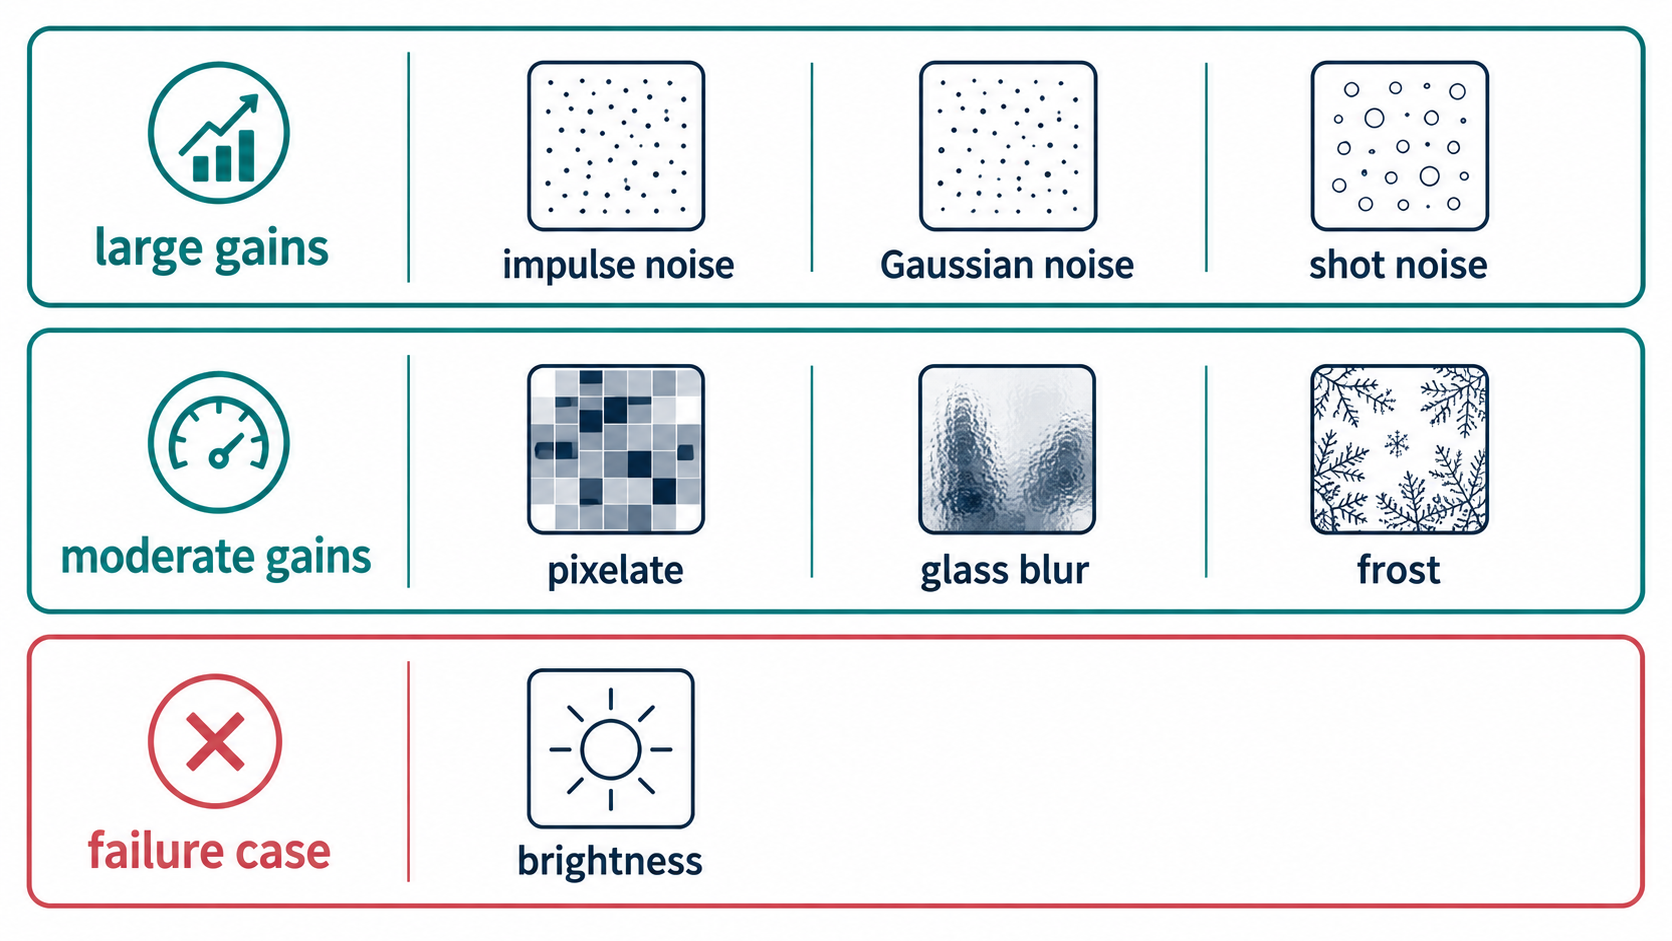
\includegraphics[width=\linewidth,height=0.58\textheight,keepaspectratio]{assets/6.png}
\end{column}
\end{columns}
\end{frame}

% 15
\begin{frame}[label=slide15]
\slidetitle{Diagnostic Analysis: Adaptation-Step Sweep}
\begin{columns}[T,totalwidth=\linewidth]
\begin{column}{0.52\linewidth}
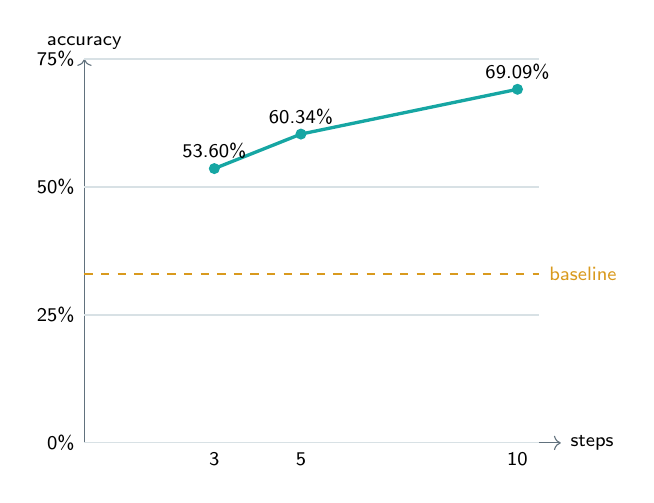
\begin{tikzpicture}[x=0.55cm,y=0.065cm]
\draw[->,draw=Muted] (0,0) -- (11,0) node[right]{\scriptsize steps};
\draw[->,draw=Muted] (0,0) -- (0,75) node[above]{\scriptsize accuracy};
\foreach \y in {0,25,50,75}{\draw[draw=Line] (0,\y)--(10.5,\y); \node[left] at (0,\y){\scriptsize \y\%};}
\draw[Gold,thick,dashed] (0,33.02)--(10.5,33.02) node[right]{\scriptsize baseline};
\draw[Teal,very thick] (3,53.60)--(5,60.34)--(10,69.09);
\foreach \x/\y/\lab in {3/53.60/53.60,5/60.34/60.34,10/69.09/69.09}{\fill[Teal] (\x,\y) circle (2pt); \node[above] at (\x,\y){\scriptsize \lab\%};}
\foreach \x in {3,5,10}{\node[below] at (\x,0){\scriptsize \x};}
\end{tikzpicture}
\end{column}
\begin{column}{0.44\linewidth}
\begin{itemize}\setlength\itemsep{0.24cm}
\item Sweep performed on \texttt{shot\_noise}, severity 5.
\item Accuracy rises from 53.60\% at 3 steps to 69.09\% at 10 steps.
\item The repository reports no rejected batches in this sweep.
\item No runtime/latency measurements are provided.
\end{itemize}
\end{column}
\end{columns}
\end{frame}

% 16
\begin{frame}[label=slide16]
\slidetitle{Failure Cases and Limitations}
\begin{columns}[T,totalwidth=\linewidth]
\begin{column}{0.49\linewidth}
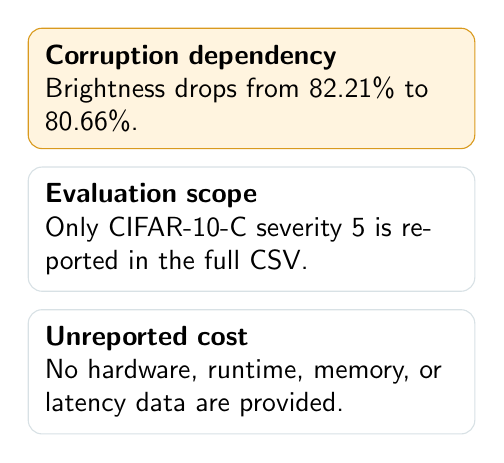
\begin{tikzpicture}[node distance=0.22cm]
\node[draw=Gold,rounded corners=5pt,fill=SoftGold,text width=5.25cm,minimum height=1.18cm,inner sep=6pt,align=left] (a) {\textbf{Corruption dependency}\\Brightness drops from 82.21\% to 80.66\%.};
\node[draw=Line,rounded corners=5pt,fill=white,text width=5.25cm,minimum height=1.18cm,inner sep=6pt,align=left,below=of a] (b) {\textbf{Evaluation scope}\\Only CIFAR-10-C severity 5 is reported in the full CSV.};
\node[draw=Line,rounded corners=5pt,fill=white,text width=5.25cm,minimum height=1.18cm,inner sep=6pt,align=left,below=of b] (c) {\textbf{Unreported cost}\\No hardware, runtime, memory, or latency data are provided.};
\end{tikzpicture}
\end{column}
\begin{column}{0.47\linewidth}
\begin{itemize}\setlength\itemsep{0.25cm}
\item The method deep-copies the model per target batch inside the adapter.
\item Only normalization parameters are adapted; this is controlled but limited.
\item No multiple-seed statistical confidence interval is reported.
\item Failure analysis is quantitative, not qualitative at image level.
\end{itemize}
\end{column}
\end{columns}
\end{frame}

% 17
\begin{frame}[label=slide17]
\slidetitle{Future Work}
\begin{columns}[T,totalwidth=\linewidth]
\begin{column}{0.49\linewidth}
\begin{enumerate}\setlength\itemsep{0.23cm}
\item Add runtime and memory profiling for each TTT step count.
\item Report multi-seed mean and standard deviation.
\item Add a safety gate for harmful shifts such as brightness.
\item Extend evaluation to lower severities and combined corruptions.
\end{enumerate}
\end{column}
\begin{column}{0.47\linewidth}
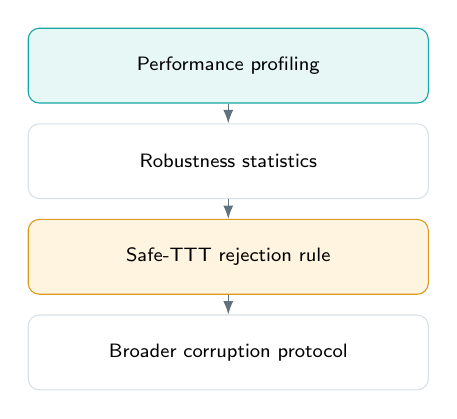
\begin{tikzpicture}[node distance=0.25cm]
\node[tealblock,text width=4.8cm] (a) {Performance profiling};
\node[block,text width=4.8cm,below=of a] (b) {Robustness statistics};
\node[goldblock,text width=4.8cm,below=of b] (c) {Safe-TTT rejection rule};
\node[block,text width=4.8cm,below=of c] (d) {Broader corruption protocol};
\draw[thinarrow] (a)--(b);\draw[thinarrow] (b)--(c);\draw[thinarrow] (c)--(d);
\end{tikzpicture}
\end{column}
\end{columns}
\vfill
\small These extensions follow directly from the repository outputs and current missing evidence.
\end{frame}

% 18
\begin{frame}[label=slide18]
\slidetitle{Engineering Contribution}
\begin{columns}[T,totalwidth=\linewidth]
\begin{column}{0.32\linewidth}\metriccard{\linewidth}{Unified experiment entry point}{run.py}\end{column}
\begin{column}{0.32\linewidth}\metriccard{\linewidth}{Reusable ML modules}{src/}\end{column}
\begin{column}{0.32\linewidth}\metriccard{\linewidth}{Evaluation outputs}{CSV logs}\end{column}
\end{columns}
\vspace{0.6cm}
\begin{columns}[T,totalwidth=\linewidth]
\begin{column}{0.38\linewidth}
{\small
\begin{itemize}\setlength\itemsep{0.22cm}
\item Config-driven SSL and TTT workflows.
\item Artifact dependency checks before TTT execution.
\item Data loaders for CIFAR-10, CIFAR-10-C, and optional rotation shift.
\item Scripts for all-corruption evaluation and adaptation-step sweep.
\end{itemize}
}
\end{column}
\begin{column}{0.58\linewidth}
\centering
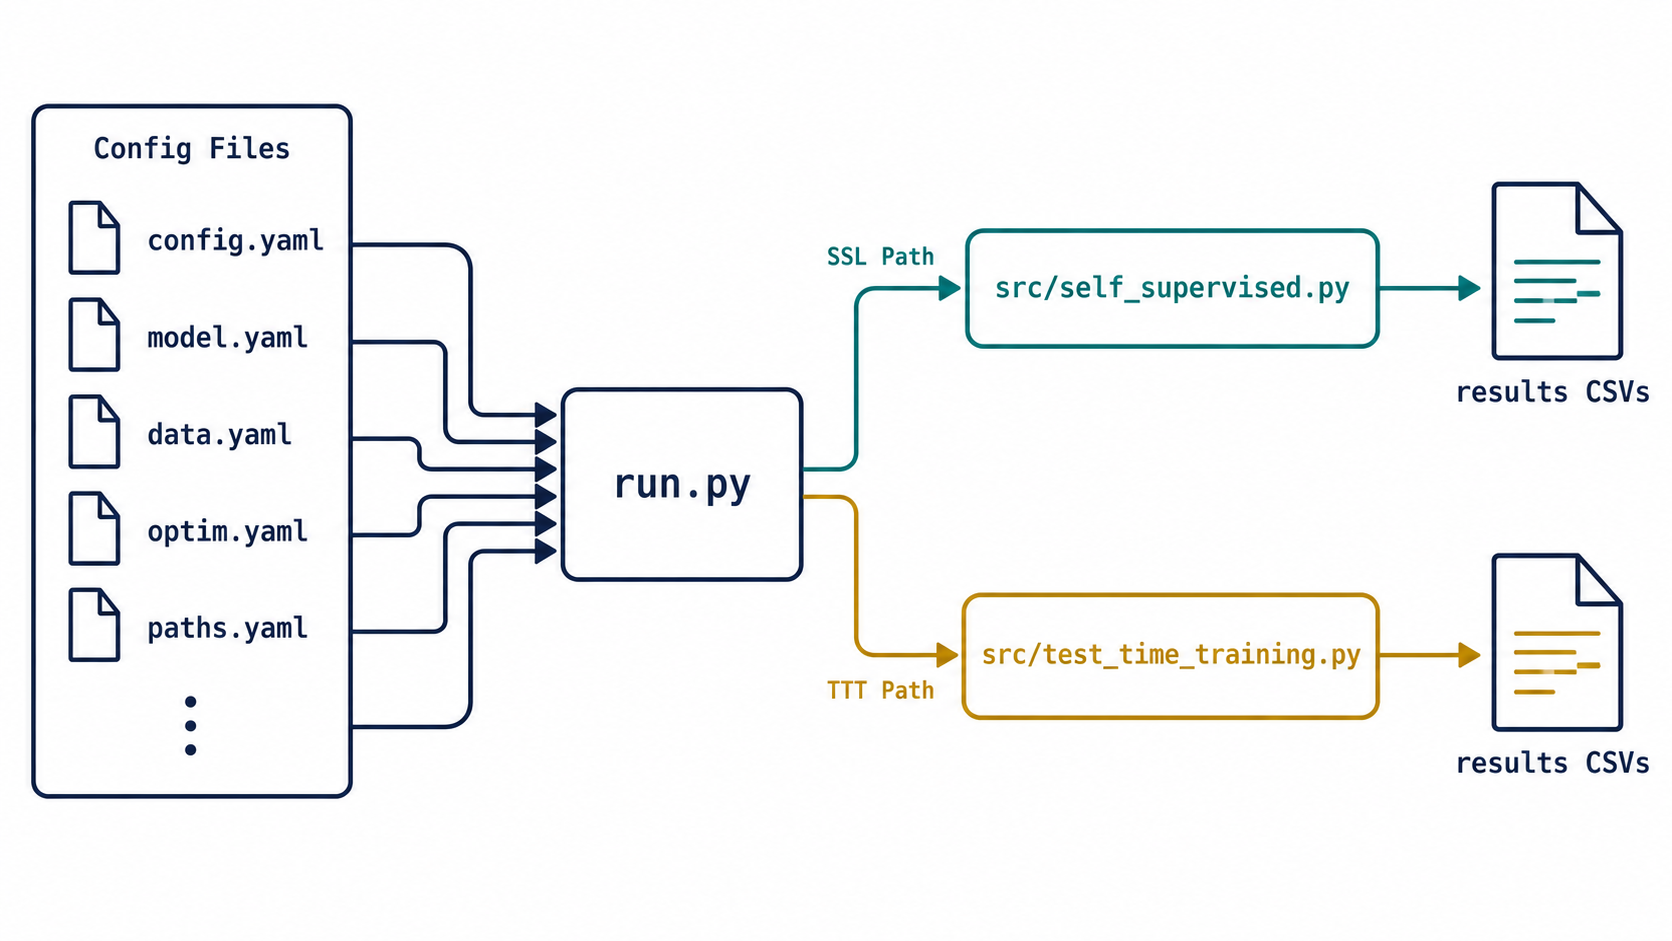
\includegraphics[width=\linewidth,height=0.58\textheight,keepaspectratio]{assets/7.png}
\end{column}
\end{columns}
\end{frame}

% 19
\begin{frame}[label=slide19]
\slidetitle{Scientific and Academic Contribution}
\begin{columns}[T,totalwidth=\linewidth]
\begin{column}{0.54\linewidth}
\begin{itemize}\setlength\itemsep{0.28cm}
\item Tests whether self-supervised source features can support unlabeled test-time adaptation.
\item Implements activation-statistic matching as a concrete TTT mechanism.
\item Provides empirical evidence across 15 corruption types, not a single cherry-picked case.
\item Identifies a real limitation: brightness shift can degrade after adaptation.
\end{itemize}
\end{column}
\begin{column}{0.42\linewidth}
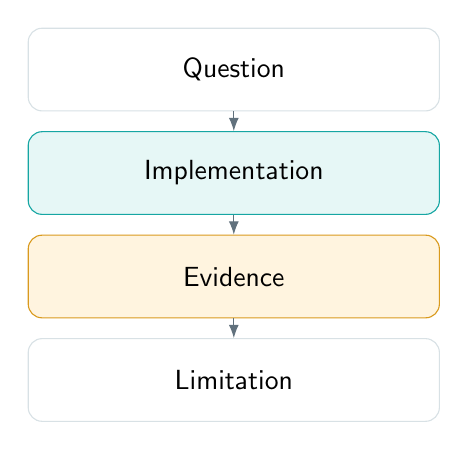
\begin{tikzpicture}
\node[draw=Line,rounded corners=5pt,fill=white,text width=4.8cm,minimum height=1.05cm,inner sep=6pt,align=center] (a) {Question};
\node[draw=Teal,rounded corners=5pt,fill=SoftTeal,text width=4.8cm,minimum height=1.05cm,inner sep=6pt,align=center,below=0.25cm of a] (b) {Implementation};
\node[draw=Gold,rounded corners=5pt,fill=SoftGold,text width=4.8cm,minimum height=1.05cm,inner sep=6pt,align=center,below=0.25cm of b] (c) {Evidence};
\node[draw=Line,rounded corners=5pt,fill=white,text width=4.8cm,minimum height=1.05cm,inner sep=6pt,align=center,below=0.25cm of c] (d) {Limitation};
\draw[thinarrow] (a)--(b);\draw[thinarrow] (b)--(c);\draw[thinarrow] (c)--(d);
\end{tikzpicture}
\end{column}
\end{columns}
\end{frame}

% 20
\begin{frame}[label=slide20]
\vspace{0.12cm}
\begin{center}
{\Large\bfseries Final Conclusion}\\[0.25cm]
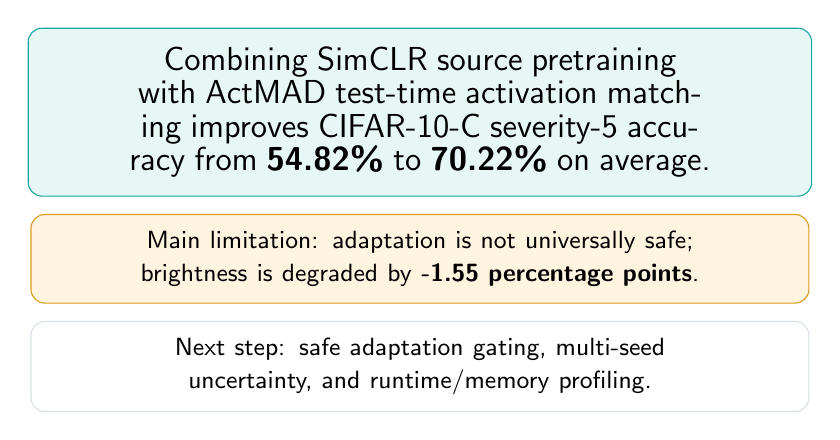
\begin{tikzpicture}[node distance=0.22cm]
\node[draw=Teal,rounded corners=5pt,fill=SoftTeal,text width=0.78\linewidth,minimum height=1.05cm,inner sep=7pt,align=center] (c1) {
\large Combining SimCLR source pretraining with ActMAD test-time activation matching improves CIFAR-10-C severity-5 accuracy from \textbf{54.82\%} to \textbf{70.22\%} on average.
};
\node[draw=Gold,rounded corners=5pt,fill=SoftGold,text width=0.78\linewidth,minimum height=0.85cm,inner sep=6pt,align=center,below=of c1] (c2) {
\small Main limitation: adaptation is not universally safe; brightness is degraded by \textbf{-1.55 percentage points}.
};
\node[draw=Line,rounded corners=5pt,fill=white,text width=0.78\linewidth,minimum height=0.85cm,inner sep=6pt,align=center,below=of c2] (c3) {
\small Next step: safe adaptation gating, multi-seed uncertainty, and runtime/memory profiling.
};
\end{tikzpicture}\\[0.22cm]

\includegraphics[width=0.17\linewidth]{assets/universite_paris_cite_logo.png}\\[0.08cm]
{\small \repo}
\end{center}
\end{frame}

% 21
\begin{frame}[label=slide21]
\slidetitle{Appendix: Numbers and Comparison}
{\scriptsize
\renewcommand{\arraystretch}{1.18}
\begin{tabularx}{\linewidth}{>{\bfseries}p{1.25cm}p{2.45cm}Y}
\toprule
Number & Domain & Meaning \\
\midrule
84.23\% & clean CIFAR-10 & Linear evaluation: frozen SimCLR backbone plus trained linear classifier on clean data. \\
54.82\% & CIFAR-10-C & Mean baseline accuracy across 15 corruptions at severity 5, before adaptation. \\
70.22\% & CIFAR-10-C & Mean ActMAD accuracy across the same 15 corruptions at severity 5, after adaptation. \\
69.09\% & shot\_noise only & One step-sweep result for shot\_noise, severity 5, with 10 adaptation steps. \\
\bottomrule
\end{tabularx}
}
\vspace{0.18cm}
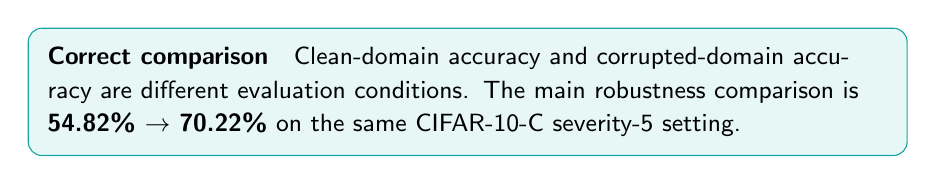
\begin{tikzpicture}
\node[draw=Teal,rounded corners=5pt,fill=SoftTeal,text width=0.88\linewidth,inner sep=7pt,align=left] {
\small\RaggedRight \textbf{Correct comparison}\quad Clean-domain accuracy and corrupted-domain accuracy are different evaluation conditions. The main robustness comparison is \textbf{54.82\% $\rightarrow$ 70.22\%} on the same CIFAR-10-C severity-5 setting.
};
\end{tikzpicture}
\end{frame}

% 22
\begin{frame}[label=slide22]
\slidetitle{Appendix: Main Result}
\begin{columns}[T,totalwidth=\linewidth]
\begin{column}{0.58\linewidth}
{\small\bfseries Main result: average over CIFAR-10-C}\\[0.16cm]
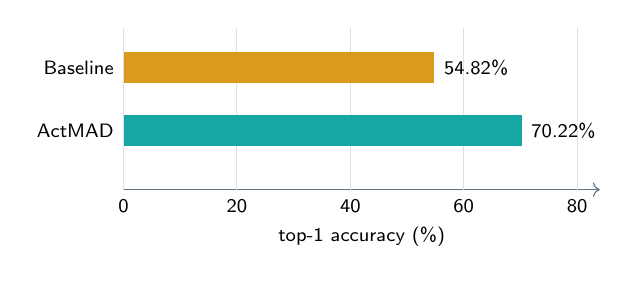
\begin{tikzpicture}[x=0.072cm,y=1cm]
\draw[->,draw=Muted] (0,0) -- (84,0);
\foreach \x in {0,20,40,60,80}{\draw[draw=Line] (\x,0) -- (\x,2.05); \node[below] at (\x,0) {\scriptsize \x};}
\fill[Gold] (0,1.35) rectangle (54.82,1.75);
\fill[Teal] (0,0.55) rectangle (70.22,0.95);
\node[left] at (0,1.55) {\scriptsize Baseline};
\node[left] at (0,0.75) {\scriptsize ActMAD};
\node[right] at (54.82,1.55) {\scriptsize 54.82\%};
\node[right] at (70.22,0.75) {\scriptsize 70.22\%};
\node[below=0.35cm] at (42,0) {\scriptsize top-1 accuracy (\%)};
\end{tikzpicture}
\end{column}
\begin{column}{0.38\linewidth}
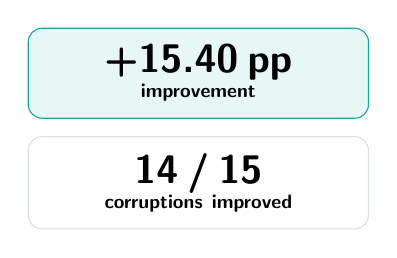
\begin{tikzpicture}[node distance=0.22cm]
\node[draw=Teal,rounded corners=5pt,fill=SoftTeal,text width=3.9cm,minimum height=1.0cm,inner sep=6pt,align=center] (a) {\Large\bfseries +15.40 pp\\[-1mm]\scriptsize improvement};
\node[draw=Line,rounded corners=5pt,fill=white,text width=3.9cm,minimum height=1.0cm,inner sep=6pt,align=center,below=of a] (b) {\Large\bfseries 14 / 15\\[-1mm]\scriptsize corruptions improved};
\end{tikzpicture}
\end{column}
\end{columns}
\vspace{0.24cm}
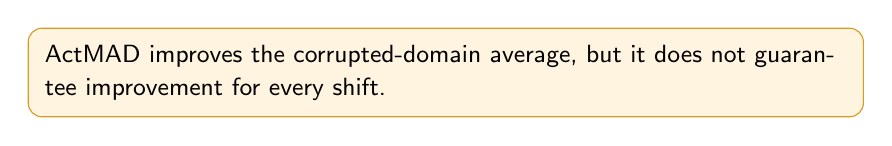
\begin{tikzpicture}
\node[draw=Gold,rounded corners=5pt,fill=SoftGold,text width=0.84\linewidth,inner sep=6pt,align=left] {
\small\RaggedRight ActMAD improves the corrupted-domain average, but it does not guarantee improvement for every shift.
};
\end{tikzpicture}
\end{frame}

% 23
\begin{frame}[label=slide23]
\slidetitle{Appendix: Per-Corruption Behavior}
{\scriptsize Accuracy gain in percentage points: ActMAD minus baseline}\\[-0.08cm]
\begin{center}
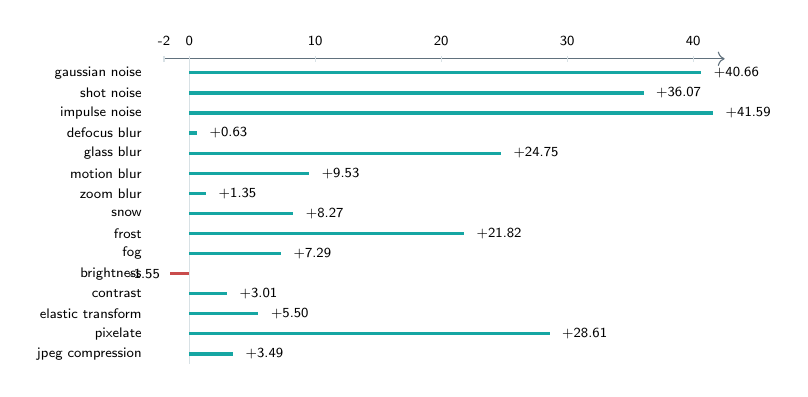
\begin{tikzpicture}[x=0.16cm,y=0.255cm,font=\tiny]
\draw[draw=Line] (0,0.5) -- (0,15.7);
\draw[->,draw=Muted] (-2,15.7) -- (42.5,15.7);
\foreach \x in {-2,0,10,20,30,40}{
  \draw[draw=Line] (\x,15.55) -- (\x,15.85);
  \node[above] at (\x,15.85) {\x};
}
\foreach \name/\val/\lab/\clr [count=\i] in {
gaussian noise/40.66/+40.66/Teal,
shot noise/36.07/+36.07/Teal,
impulse noise/41.59/+41.59/Teal,
defocus blur/0.63/+0.63/Teal,
glass blur/24.75/+24.75/Teal,
motion blur/9.53/+9.53/Teal,
zoom blur/1.35/+1.35/Teal,
snow/8.27/+8.27/Teal,
frost/21.82/+21.82/Teal,
fog/7.29/+7.29/Teal,
brightness/-1.55/-1.55/Danger,
contrast/3.01/+3.01/Teal,
elastic transform/5.50/+5.50/Teal,
pixelate/28.61/+28.61/Teal,
jpeg compression/3.49/+3.49/Teal}{
  \pgfmathsetmacro{\y}{16-\i}
  \node[anchor=east] at (-3,\y) {\name};
  \ifdim\val pt>0pt
    \fill[\clr] (0,\y-0.08) rectangle (\val,\y+0.08);
    \node[anchor=west] at (\val,\y) {\hspace{1pt}\lab};
  \else
    \fill[\clr] (\val,\y-0.08) rectangle (0,\y+0.08);
    \node[anchor=east] at (\val,\y) {\lab\hspace{1pt}};
  \fi
}
\end{tikzpicture}
\end{center}
\vspace{-0.12cm}
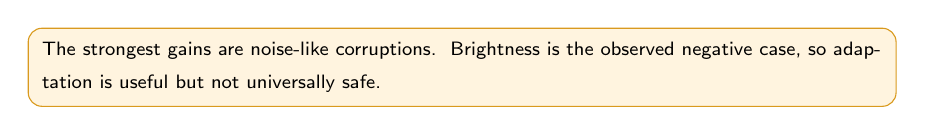
\begin{tikzpicture}
\node[draw=Gold,rounded corners=5pt,fill=SoftGold,text width=0.88\linewidth,inner sep=5pt,align=left] {
\scriptsize\RaggedRight The strongest gains are noise-like corruptions. Brightness is the observed negative case, so adaptation is useful but not universally safe.
};
\end{tikzpicture}
\end{frame}

% 24
\begin{frame}[label=slide24]
\slidetitle{Appendix: Shot-Noise Step Sweep}
\begin{columns}[T,totalwidth=\linewidth]
\begin{column}{0.57\linewidth}
{\small\bfseries Step sweep: shot\_noise only}\\[0.1cm]
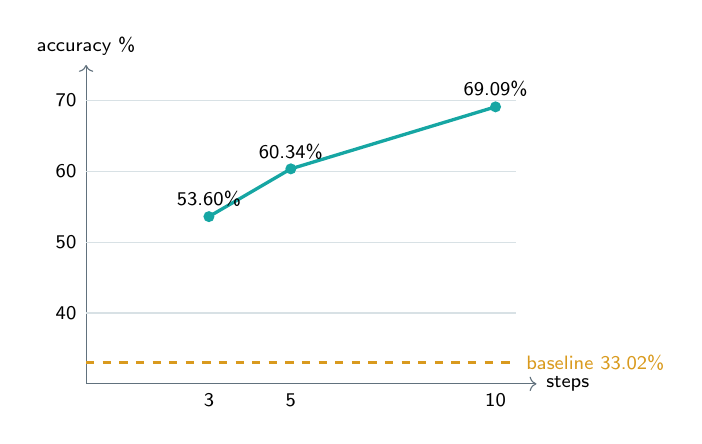
\begin{tikzpicture}[x=0.52cm,y=0.09cm,font=\scriptsize]
\draw[->,draw=Muted] (0,30) -- (11,30) node[right]{steps};
\draw[->,draw=Muted] (0,30) -- (0,75) node[above]{accuracy \%};
\foreach \y in {40,50,60,70}{
  \draw[draw=Line] (0,\y)--(10.5,\y);
  \node[left] at (0,\y){\y};
}
\draw[Gold,thick,dashed] (0,33.02)--(10.5,33.02) node[right]{baseline 33.02\%};
\draw[Teal,very thick] (3,53.60)--(5,60.34)--(10,69.09);
\foreach \x/\y/\lab in {3/53.60/53.60\%,5/60.34/60.34\%,10/69.09/69.09\%}{
  \fill[Teal] (\x,\y) circle (2pt);
  \node[above] at (\x,\y){\lab};
}
\foreach \x in {3,5,10}{\node[below] at (\x,30){\x};}
\end{tikzpicture}
\end{column}
\begin{column}{0.39\linewidth}
{\scriptsize
\renewcommand{\arraystretch}{1.18}
\begin{tabular}{@{}>{\bfseries}p{1.7cm}r@{}}
\toprule
Setting & Accuracy \\
\midrule
Baseline & 33.02\% \\
3 steps & 53.60\% \\
5 steps & 60.34\% \\
10 steps & 69.09\% \\
\bottomrule
\end{tabular}
}
\vspace{0.25cm}
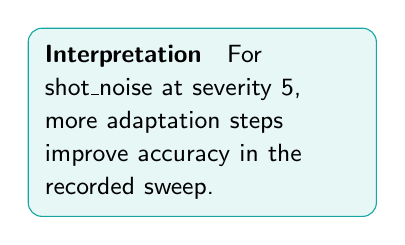
\begin{tikzpicture}
\node[draw=Teal,rounded corners=5pt,fill=SoftTeal,text width=4.0cm,inner sep=6pt,align=left] {
\small \textbf{Interpretation}\quad For shot\_noise at severity 5, more adaptation steps improve accuracy in the recorded sweep.
};
\end{tikzpicture}
\end{column}
\end{columns}
\end{frame}

\end{document}
